\documentclass{standalone}
\usepackage{tikz}
\usetikzlibrary{patterns, positioning}


\begin{document}
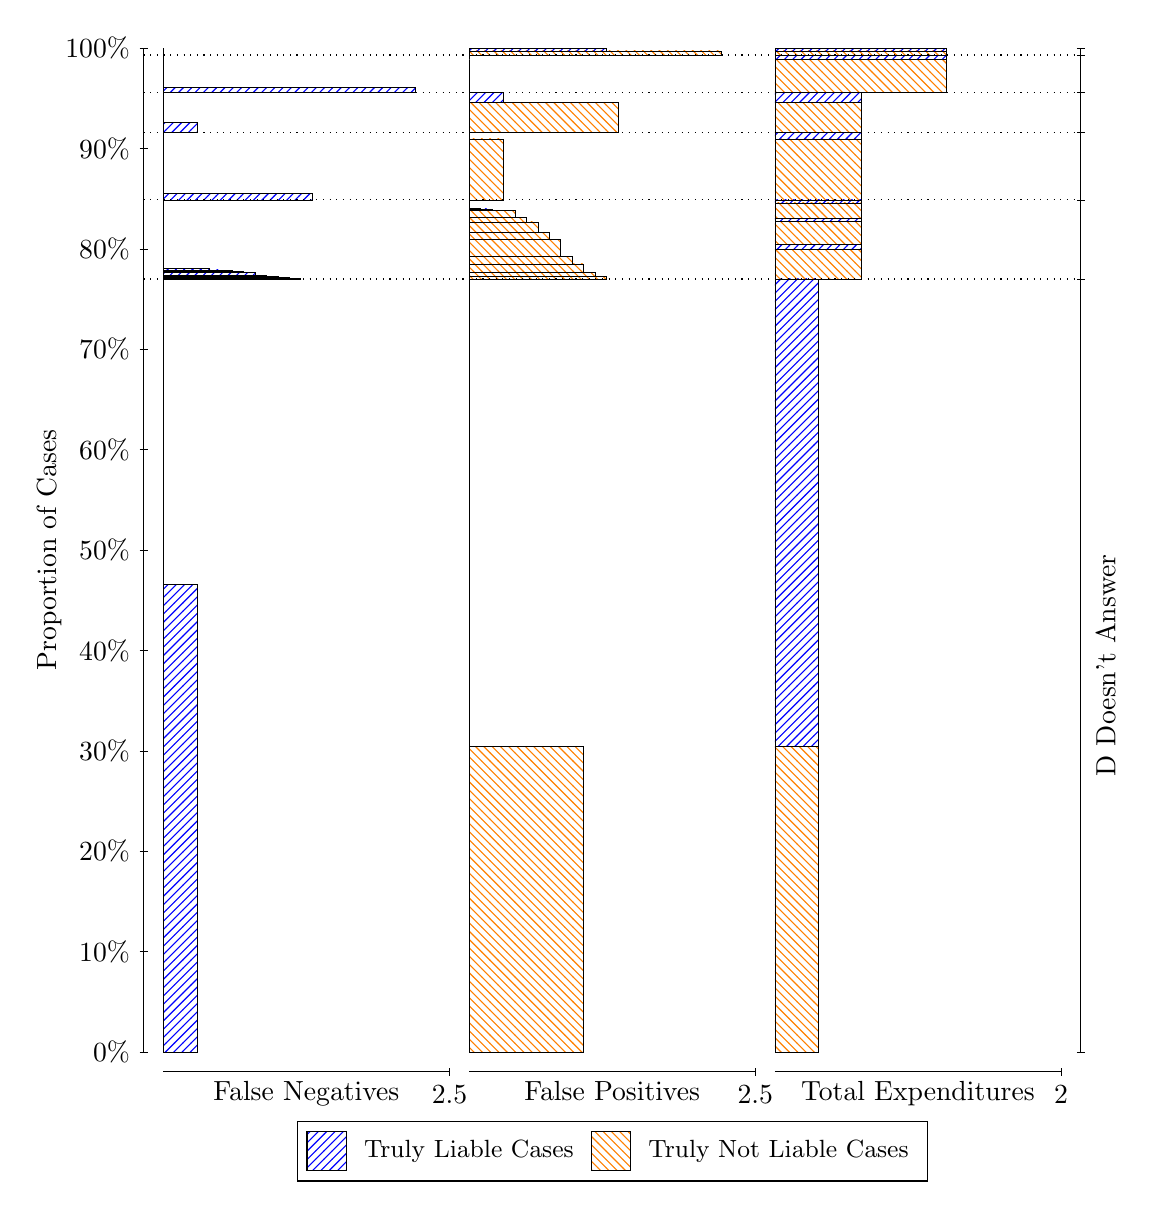
\begin{tikzpicture}
\draw[black, very thin] (1.5,1.75) -- (1.5,14.5);
\node[rotate=90, text=black, anchor=center] at (0.3, 8.125) {Proportion of Cases};
\draw[black, very thin] (1.45,1.75) -- (1.55,1.75);
\node[text=black, anchor=east] at (1.45, 1.75) {0\%};
\draw[black, very thin] (1.45,3.025) -- (1.55,3.025);
\node[text=black, anchor=east] at (1.45, 3.025) {10\%};
\draw[black, very thin] (1.45,4.3) -- (1.55,4.3);
\node[text=black, anchor=east] at (1.45, 4.3) {20\%};
\draw[black, very thin] (1.45,5.575) -- (1.55,5.575);
\node[text=black, anchor=east] at (1.45, 5.575) {30\%};
\draw[black, very thin] (1.45,6.85) -- (1.55,6.85);
\node[text=black, anchor=east] at (1.45, 6.85) {40\%};
\draw[black, very thin] (1.45,8.125) -- (1.55,8.125);
\node[text=black, anchor=east] at (1.45, 8.125) {50\%};
\draw[black, very thin] (1.45,9.4) -- (1.55,9.4);
\node[text=black, anchor=east] at (1.45, 9.4) {60\%};
\draw[black, very thin] (1.45,10.675) -- (1.55,10.675);
\node[text=black, anchor=east] at (1.45, 10.675) {70\%};
\draw[black, very thin] (1.45,11.95) -- (1.55,11.95);
\node[text=black, anchor=east] at (1.45, 11.95) {80\%};
\draw[black, very thin] (1.45,13.225) -- (1.55,13.225);
\node[text=black, anchor=east] at (1.45, 13.225) {90\%};
\draw[black, very thin] (1.45,14.5) -- (1.55,14.5);
\node[text=black, anchor=east] at (1.45, 14.5) {100\%};

\draw[black, very thin] (13.4,1.75) -- (13.4,14.5);
\draw[black, very thin] (13.35,1.75) -- (13.45,1.75);
\node[anchor=west] at (13.35, 1.75) {};
\draw[black, very thin] (13.35,11.567) -- (13.45,11.567);
\node[anchor=west] at (13.35, 11.567) {};
\draw[black, very thin] (13.35,12.571) -- (13.45,12.571);
\node[anchor=west] at (13.35, 12.571) {};
\draw[black, very thin] (13.35,13.429) -- (13.45,13.429);
\node[anchor=west] at (13.35, 13.429) {};
\draw[black, very thin] (13.35,13.94) -- (13.45,13.94);
\node[anchor=west] at (13.35, 13.94) {};
\draw[black, very thin] (13.35,14.411) -- (13.45,14.411);
\node[anchor=west] at (13.35, 14.411) {};
\draw[black, very thin] (13.35,14.5) -- (13.45,14.5);
\node[anchor=west] at (13.35, 14.5) {};

\draw[black, very thin, pattern color=blue, pattern=north east lines] (1.75,1.75) rectangle (2.186,7.6906);
\draw[black, very thin, pattern color=orange, pattern=north west lines] (1.75,7.6906) rectangle (1.75,11.567);
\draw[black, very thin, pattern color=blue, pattern=north east lines] (1.75,11.567) rectangle (3.494,11.577);
\draw[black, very thin, pattern color=blue, pattern=north east lines] (1.75,11.577) rectangle (3.3487,11.583);
\draw[black, very thin, pattern color=blue, pattern=north east lines] (1.75,11.583) rectangle (3.2033,11.598);
\draw[black, very thin, pattern color=blue, pattern=north east lines] (1.75,11.598) rectangle (3.058,11.601);
\draw[black, very thin, pattern color=blue, pattern=north east lines] (1.75,11.601) rectangle (3.058,11.611);
\draw[black, very thin, pattern color=blue, pattern=north east lines] (1.75,11.611) rectangle (2.9127,11.647);
\draw[black, very thin, pattern color=blue, pattern=north east lines] (1.75,11.647) rectangle (2.7673,11.659);
\draw[black, very thin, pattern color=blue, pattern=north east lines] (1.75,11.659) rectangle (2.622,11.675);
\draw[black, very thin, pattern color=blue, pattern=north east lines] (1.75,11.675) rectangle (2.4767,11.683);
\draw[black, very thin, pattern color=blue, pattern=north east lines] (1.75,11.683) rectangle (2.3313,11.698);
\draw[black, very thin, pattern color=orange, pattern=north west lines] (1.75,11.698) rectangle (1.75,12.571);
\draw[black, very thin, pattern color=blue, pattern=north east lines] (1.75,12.571) rectangle (3.6393,12.655);
\draw[black, very thin, pattern color=orange, pattern=north west lines] (1.75,12.655) rectangle (1.75,13.429);
\draw[black, very thin, pattern color=blue, pattern=north east lines] (1.75,13.429) rectangle (2.186,13.559);
\draw[black, very thin, pattern color=orange, pattern=north west lines] (1.75,13.559) rectangle (1.75,13.94);
\draw[black, very thin, pattern color=blue, pattern=north east lines] (1.75,13.94) rectangle (4.9473,13.996);
\draw[black, very thin, pattern color=orange, pattern=north west lines] (1.75,13.996) rectangle (1.75,14.411);
\draw[black, very thin, pattern color=orange, pattern=north west lines] (1.75,14.411) rectangle (1.75,14.465);
\draw[black, very thin, pattern color=blue, pattern=north east lines] (1.75,14.465) rectangle (1.75,14.5);
\draw[black, very thin, pattern color=orange, pattern=north west lines] (5.6333,1.75) rectangle (7.0867,5.6268);
\draw[black, very thin, pattern color=blue, pattern=north east lines] (5.6333,5.6268) rectangle (5.6333,11.567);
\draw[black, very thin, pattern color=orange, pattern=north west lines] (5.6333,11.567) rectangle (7.3773,11.603);
\draw[black, very thin, pattern color=orange, pattern=north west lines] (5.6333,11.603) rectangle (7.232,11.649);
\draw[black, very thin, pattern color=orange, pattern=north west lines] (5.6333,11.649) rectangle (7.0867,11.76);
\draw[black, very thin, pattern color=orange, pattern=north west lines] (5.6333,11.76) rectangle (6.9413,11.852);
\draw[black, very thin, pattern color=orange, pattern=north west lines] (5.6333,11.852) rectangle (6.796,12.074);
\draw[black, very thin, pattern color=orange, pattern=north west lines] (5.6333,12.074) rectangle (6.6507,12.163);
\draw[black, very thin, pattern color=orange, pattern=north west lines] (5.6333,12.163) rectangle (6.5053,12.293);
\draw[black, very thin, pattern color=orange, pattern=north west lines] (5.6333,12.293) rectangle (6.36,12.346);
\draw[black, very thin, pattern color=orange, pattern=north west lines] (5.6333,12.346) rectangle (6.2147,12.441);
\draw[black, very thin, pattern color=blue, pattern=north east lines] (5.6333,12.441) rectangle (5.924,12.456);
\draw[black, very thin, pattern color=blue, pattern=north east lines] (5.6333,12.456) rectangle (5.7787,12.464);
\draw[black, very thin, pattern color=blue, pattern=north east lines] (5.6333,12.464) rectangle (5.6333,12.571);
\draw[black, very thin, pattern color=orange, pattern=north west lines] (5.6333,12.571) rectangle (6.0693,13.346);
\draw[black, very thin, pattern color=blue, pattern=north east lines] (5.6333,13.346) rectangle (5.6333,13.429);
\draw[black, very thin, pattern color=orange, pattern=north west lines] (5.6333,13.429) rectangle (7.5227,13.811);
\draw[black, very thin, pattern color=blue, pattern=north east lines] (5.6333,13.811) rectangle (6.0693,13.94);
\draw[black, very thin, pattern color=orange, pattern=north west lines] (5.6333,13.94) rectangle (5.6333,14.355);
\draw[black, very thin, pattern color=blue, pattern=north east lines] (5.6333,14.355) rectangle (5.6333,14.411);
\draw[black, very thin, pattern color=orange, pattern=north west lines] (5.6333,14.411) rectangle (8.8307,14.465);
\draw[black, very thin, pattern color=blue, pattern=north east lines] (5.6333,14.465) rectangle (7.3773,14.5);
\draw[black, very thin, pattern color=orange, pattern=north west lines] (9.5167,1.75) rectangle (10.062,5.6268);
\draw[black, very thin, pattern color=blue, pattern=north east lines] (9.5167,5.6268) rectangle (10.062,11.567);
\draw[black, very thin, pattern color=orange, pattern=north west lines] (9.5167,11.567) rectangle (10.607,11.947);
\draw[black, very thin, pattern color=blue, pattern=north east lines] (9.5167,11.947) rectangle (10.607,12.006);
\draw[black, very thin, pattern color=orange, pattern=north west lines] (9.5167,12.006) rectangle (10.607,12.301);
\draw[black, very thin, pattern color=blue, pattern=north east lines] (9.5167,12.301) rectangle (10.607,12.334);
\draw[black, very thin, pattern color=orange, pattern=north west lines] (9.5167,12.334) rectangle (10.607,12.534);
\draw[black, very thin, pattern color=blue, pattern=north east lines] (9.5167,12.534) rectangle (10.607,12.571);
\draw[black, very thin, pattern color=orange, pattern=north west lines] (9.5167,12.571) rectangle (10.607,13.346);
\draw[black, very thin, pattern color=blue, pattern=north east lines] (9.5167,13.346) rectangle (10.607,13.429);
\draw[black, very thin, pattern color=orange, pattern=north west lines] (9.5167,13.429) rectangle (10.607,13.811);
\draw[black, very thin, pattern color=blue, pattern=north east lines] (9.5167,13.811) rectangle (10.607,13.94);
\draw[black, very thin, pattern color=orange, pattern=north west lines] (9.5167,13.94) rectangle (11.697,14.355);
\draw[black, very thin, pattern color=blue, pattern=north east lines] (9.5167,14.355) rectangle (11.697,14.411);
\draw[black, very thin, pattern color=orange, pattern=north west lines] (9.5167,14.411) rectangle (11.697,14.465);
\draw[black, very thin, pattern color=blue, pattern=north east lines] (9.5167,14.465) rectangle (11.697,14.5);
\draw[black, dotted] (1.5,11.567) -- (13.4,11.567);
\draw[black, dotted] (1.5,12.571) -- (13.4,12.571);
\draw[black, dotted] (1.5,13.429) -- (13.4,13.429);
\draw[black, dotted] (1.5,13.94) -- (13.4,13.94);
\draw[black, dotted] (1.5,14.411) -- (13.4,14.411);
\draw[black, very thin] (1.75,1.5) -- (5.3833,1.5);
\node[text=black, anchor=north] at (3.5667, 1.5) {False Negatives};
\draw[black, very thin] (5.3833,1.45) -- (5.3833,1.55);
\node[text=black, anchor=north] at (5.3833, 1.45) {2.5};

\draw[black, very thin] (5.6333,1.5) -- (9.2667,1.5);
\node[text=black, anchor=north] at (7.45, 1.5) {False Positives};
\draw[black, very thin] (9.2667,1.45) -- (9.2667,1.55);
\node[text=black, anchor=north] at (9.2667, 1.45) {2.5};

\draw[black, very thin] (9.5167,1.5) -- (13.15,1.5);
\node[text=black, anchor=north] at (11.333, 1.5) {Total Expenditures};
\draw[black, very thin] (13.15,1.45) -- (13.15,1.55);
\node[text=black, anchor=north] at (13.15, 1.45) {2};

\node[text=black, centered, rotate=90] at (13.72, 6.6587) {D Doesn't Answer};






\draw (7.449999999999999,1.5) node[draw=none] (baseCoordinate) {};
\begin{scope}[align=center]
        \matrix[scale=0.5, draw=black, below=0.5cm of baseCoordinate, nodes={draw}, column sep=0.1cm]{
            \node[rectangle, draw, minimum width=0.5cm, minimum height=0.5cm, pattern color=blue, pattern=north east lines] {}; &
            \node[draw=none, font=\small, text=black] (B) {Truly Liable Cases}; &
            \node[rectangle, draw, minimum width=0.5cm, minimum height=0.5cm, pattern color=orange, pattern=north west lines] {}; &
            \node[draw=none, font=\small, text=black] (B) {Truly Not Liable Cases}; \\
            };
\end{scope}

\end{tikzpicture}
\end{document}